\chapter{Advancements to the EXPRES Pipeline} \label{chapter:pipeline2}

\section{Introduction}

After the completion of the EXPRES pipeline and the presentation of initial results as described in Chapter \ref{chapter:pipeline}, there remained many possibilities for further improvement to the reliability and accuracy of the pipeline. Although the resultant RVs yield statistical precision around 30\cms that varies consistently with the measured signal-to-noise as shown in the previous chapter, residual RMS compared to fit Keplerian orbits still hover around the 1\ms level for HD 217014 \citep{petersburg_extreme-precision_2020} and 58\cms level for HD 3651 \citep{brewer_expres_2020}. Naturally, these levels of precision set a new standard for RV measurement in the community, but they still do not reach the expected instrumental precision determined by \citet{blackman_performance_2020} of 30\cms. Thus, I expected that improvements could nevertheless be made to the pipeline in order to push this standard even further.

In this chapter, I detail contributions I made to the pipeline beyond what was presented in the previous chapter in three separate areas. The first (Chapter \ref{pipeline2:spec-perf}) is the introduction of spectro-perfectionism to the pipeline as a step into an extra dimension of analysis as compared to optimal extraction. The second (Chapter \ref{pipeline2:bspline}) shows how \textit{B}-splines can and have been used in the pipeline to improve our understanding of the spectra that overlap adjacent \'{e}chelle orders. Finally, the third (Chapter \ref{pipeline2:forward-model}) demonstrates an application of \textit{B}-spline stellar templates as an empirical forward model to measure radial velocities.

\section{Spectro-perfectionism} \label{pipeline2:spec-perf}

Optimal extraction, even the flat-relative variety as presented in Chapter \ref{optimal-extraction}, unfortunately misses out on some information about the instrument and thus cannot maximally extract data. In particular, this is because optimal extraction extracts one column at a time across each order. This process assumes that each extract-able spectral ``bin'' is distributed only along each column without any information shared between adjacent columns on the detector.

Rather, \'{e}chelle spectrographs typically have a slit function that is wider than a single pixel on the detector and the function itself tends to have Gaussian-like tails that extend well beyond the brightest pixels of the projected slit. Therefore, there is inherent cross-talk along the columns of an extracted order: the brightness in one pixel is highly correlated with the brightness in neighboring pixels. In addition, \'{e}chelle spectrographs are typically fiber-fed, meaning the resultant point-spread function (PSF) of the instrument is sometimes non-rectangular and, even if rectangular, angled when compared to the alignment of the detector pixels.

To fully understand the potential issue with optimal extraction, consider the exaggerated example of a rectangular fiber that is 30-degrees from vertical in the reference frame of the detector. A flat field source projected through the spectrograph with this PSF configuration would be continuous, as expected from an aligned PSF. However, when taking vertical cross-sections of a stellar observation order with a deep absorption line and comparing them against this flat field calibration, as is done in optimal extraction, the shapes definitely do not match up.

Therefore, \citet{bolton_spectro-perfectionism_2009} devised \textit{spectro-perfectionism}, a numerical method that includes as much information about the PSF as possible during the extraction process. Simply, spectro-perfectionism attempts to deconvolve each \'{e}chelle order using knowledge of the 2D PSF at every position along the order trace, yielding an array of statistically uncorrelated spectral bins. Thus, implementation of spectro-perfectionism is two-fold: (1) Determination of the PSF at any position on the detector and (2) execution of the deconvolution algorithm.

In this section, I describe my own implementation of spectro-perfectionism for use in extracting EXPRES spectra. As far as I'm aware, spectro-perfectionism has only been implemented with SDSS-II \citep{bolton_spectro-perfectionism_2009} and Minerva-Red \citep{cornachione_full_2019} with results that appear comparable to those from optimal extraction. However, there are two major improvements that I present here from my work:
\begin{enumerate}
    \item The use of a ``flat-relative PSF'' and
    \item Optimizations that enable extraction of a full order simultaneously.
\end{enumerate}

A typical complaint about spectro-perfectionism is that it is limited by the ability to measure the instrument's PSF: inaccuracies in the PSF at any given position easily propagate along the order and can affect large swaths of data. Therefore, I propose using a flat-relative approach (similar to what is implemented with EXPRES's optimal extraction), which as I show in Section \ref{pipeline2:spec-perf:psf} helps by reducing the dimensionality of the problem.

Also, one possible concern I had with the implementation by \citet{cornachione_full_2019} is the fact that each order is chopped up into multiple sections during deconvolution. Considering the implications of hard borders on a deconvolution problem (see e.g. the Gibbs phenomenon), it is likely this would introduce ringing artifacts into the extracted data. As I show in Section \ref{pipeline2:spec-perf:implement}, extraction of a full order (even one nearly 8000 pixels wide) with spectro-perfectionism is computationally tractable and mitigates possible artifacting.


\subsection{The Deconvolution Problem} \label{pipeline2:spec-perf:bkgd}

In principle, \'{e}chelle spectrograph extraction is a convolution problem. The reduced (see Chapter \ref{reduction}) detector data $D_{x,y}$ with pixel indices $(x, y)$ for a given \'{e}chelle order is a convolution of the spectral intensities ($s(\lambda)$ at wavelength $\lambda$) and the instrument's wavelength-dependent PSF ($\Psi_{x,y}(\lambda)$) with added photon- and read-noise $n_{x,y}$:
\begin{equation}
    D_{x,y} = \int \Psi_{x,y}(\lambda) s(\lambda) \dd{\lambda} + n_{x,y}.
\end{equation}
\label{eq:convolution-integral}
Since the orders on the EXPRES spectrograph are spaced relatively far apart, I assume they are functionally independent in this framework. Extraction is therefore solving for $s(\lambda)$ given $D_{x,y}$ and some knowledge of $\Psi_{x,y}(\lambda)$.

In order to make Equation \ref{eq:convolution-integral} numerically tractable, it must be discretized such that $\vb{s}$ is a vector at given wavelength sampling positions {$\lambda_x$} (the $x$ here does imply that these positions relate to pixel positions, as discussed in the next section) and $\vb{\Psi}$ is a matrix with a PSF representation at each $\lambda_x$:
\begin{equation}
    D_{x,y} = \left( \sum_\lambda \Psi_{x,y,\lambda} s_\lambda \right) + n_{x,y}
    \label{eq:convolution-index}
\end{equation}
or in matrix notation
\begin{equation}
    \vb{D} = \vb{\Psi}\vb{s} + \vb{n}
    \label{eq:convolution-matrix}
\end{equation}
Note that $\Psi_{x,y}$ at any given $\lambda$ is an extremely sparse matrix, since the PSF of the instrument is much smaller than the full detector.

Solving Equation \ref{eq:convolution-matrix} is now just a matter of $\chi^2$-minimization, which is trivially
\begin{equation}
    \vb{s} = (\vb{\Psi}^\mathrm{T} \vb{\Sigma}_{\vb{D}}^{-1/2} \vb{\Psi})^{-1} \vb{\Psi}^\mathrm{T} \vb{\Sigma}_{\vb{D}}^{-1/2} \vb{D}
    \label{eq:convolution-soln}
\end{equation}
where $\vb{\Sigma_D}$ is covariance matrix for the reduced data. I assume here that $\Sigma_D$ is diagonal (in the three-dimensional sense) because the dominant detector noise properties---particularly photon- and read-noise---are uncorrelated. That being said, off-axis terms---due to e.g. pixel non-uniformity---could be included if so desired, though with a cost to complexity.

An important observation about Equation \ref{eq:convolution-soln} is that the matrix
\begin{equation}
    \vb{\Sigma_s} = (\vb{\Psi}^\mathrm{T} \vb{\Sigma}_{\vb{D}}^{-1/2} \vb{\Psi})^{-1}
\end{equation}
is the covariance matrix associated with the extracted spectrum. Except in the case of a PSF that is perfectly aligned to the columns of the detector (which is exactly the assumption made by optimal extraction), $\vb{\Sigma_s}$ is unfortunately not diagonal, meaning the individually extracted spectral values have statistically correlated uncertainty. This construction results in significant ``ringing'' in $\vb{s}$, rendering it highly unusable as a typical spectrum.

Therefore, I also use a reconvolution matrix ($\vb{R}$) to diagonalize the covariance matrix
\begin{equation}
    \vb{\Tilde{\Sigma}_s} = \vb{R} \vb{\Sigma_s} \vb{R}^\mathrm{T}
\end{equation}
and effectively convolve the spectrum back to its expected resolution
\begin{equation}
    \vb{\Tilde{s}} = \vb{R} \vb{s}
\end{equation}
thereby removing the ringing caused by Equation \ref{eq:convolution-soln} \citep{bolton_spectro-perfectionism_2009}. The full derivation for $\vb{R}$, which involves taking the matrix square root of $\vb{\Sigma_s}$ and normalizing each column, can be found in \citet{bolton_spectro-perfectionism_2009} in Section 3.

\subsection{Flat-relative Point Spread Function Modeling} \label{pipeline2:spec-perf:psf}

The first step in executing a spectro-perfectionism algorithm is determining the PSF of the instrument. Ideally, the PSF of a spectrograph would be constant across the entire CCD, immensely simplifying the computation costs of the deconvolution. However, the PSF of EXPRES (and most contemporaeneous spectrographs) changes significantly between orders and even along a single order. For example, the bluest orders on the EXPRES detector are about 2 pixels taller than the reddest orders. Thus, a parameterized PSF model is necessary to map out the PSF pixel-by-pixel.

As in previous iterations of spectro-perfectionism \citep{bolton_spectro-perfectionism_2009, cornachione_full_2019}, the EXPRES PSF model can be fully approximated using a two-dimensional function. For this, I choose a extension of the one-dimensional function presented in Chapter \ref{master-flat} used for modelling the cross-dispersion shape of the extended flat. In two dimensions, this function has the analytic form
\begin{multline}
    \Psi(x, y; A, x_0, y_0, \theta_x, \theta_y, d_x, d_y, \sigma_x, \sigma_y) = \\
    \frac{A}{4} \Bigg[\Phi\bigg(\frac{x' + d_x/2}{\sigma_x \sqrt{2}}\bigg) - \Phi\bigg(\frac{x' - d_x/2}{\sigma_x \sqrt{2}}\bigg)\Bigg] \Bigg[\Phi\bigg(\frac{y' + d_y/2}{\sigma_y \sqrt{2}}\bigg) - \Phi\bigg(\frac{y' - d_y/2}{\sigma_y \sqrt{2}}\bigg)\Bigg]
    \label{eq:expres_psf}
\end{multline}
where $\Phi(x)$ is the error function, and $x',y'$ are related to $x,y$ by a linear transformation as
\begin{equation}
    \begin{bmatrix}x' \\ y' \end{bmatrix} = 
    \begin{bmatrix}\cos \theta_x & -\sin\theta_x \\ \sin \theta_y & \cos\theta_y\end{bmatrix}\begin{bmatrix}x-x_0 \\ y-y_0\end{bmatrix}.
    \label{eq:pix-transformation}
\end{equation}

This parameterization is advantageous because it is aptly descriptive of the Fourier optics approximation introduced in Chapter \ref{master-flat}:
\begin{itemize}
    \item $x_0$ and $y_0$ are the given pixel position of the parameterized PSF,
    \item $d_x$ and $d_y$ are the dimensions of the rectangular fiber input after dispersion and cross-dispersion stretching respectively,
    \item $\sigma_x$ and $\sigma_y$ correlate with the amount of Gaussian smoothing caused by the EXPRES optics along each dimension,
    \item $\theta_x$ corresponds to the angular misalignment of the fiber input to the pixels of the detector, and
    \item $\theta_y$ corresponds to the local slope of the order trace.
\end{itemize}
Not only does this model allow us to map the PSF across the CCD with only eight parameters (and a variable amplitude), it also provides information on the magnification and de-focusing of the instrument. Also, since we expect these parameters to vary smoothly across the detector, we can more easily interpolate (and possibly extrapolate) to regions without easily measurable PSFs.

There is, however, a method to construct the PSF of EXPRES with fewer parameters and using even more information from the instrument. I call this a \textit{flat-relative} PSF, since it was influenced by the flat-relative optimal extraction work by \citet{zechmeister_flat-relative_2014} that was implemented within the EXPRES pipeline as in Chapter \ref{optimal-extraction}. The science flats provided nightly with EXPRES contain a wealth of information about the cross-dispersion PSF of the instrument as well as pixel-level variations. These qualities are what provide such an excellent one-dimensional extraction model in Chapter \ref{chapter:pipeline}, therefore it follows that the nightly flats should be useful when constructing the two-dimensional model for spectro-perfectionism.

The flat-relative two-dimensional model used with EXPRES is the product of a one-dimensional Super-Gaussian with the nightly median-combined science flat:
\begin{equation}
    \Psi(x, y; A, x_0, y_0, \theta_x, d_x, p_x) = \frac{A}{b_x} \exp{-\left(\frac{x'^2}{2\sigma_x^2}\right)^{p_x}}~F(x,y)
    \label{eq:flat-relative-psf}
\end{equation}
where
\begin{equation}
    b_x = \sqrt{2}~\frac{\sigma_x}{p_x}~\Gamma\left(\frac{1}{2 p_x}\right),
\end{equation}
\begin{equation}
    \sigma_x = \frac{d_x}{2\sqrt{2 \log{2}^{1/p_x}}},
\end{equation}
$\Gamma$ is the Gamma function, $x'$ is defined as in Equation \ref{eq:pix-transformation}, and $F(x,y)$ is the nightly reduced science flat. Note the subtle changes in variable definitions using this new form:
\begin{itemize}
    \item $d_x$ is the full width half maximum of the Super-Gaussian,
    \item $p_x$ is the power of the Super-Gaussian (a larger value means a flatter top to the PSF),
    \item $\sigma_x$ is able to be calculated directly from $d_x$ and $p_x$, and
    \item $b_x$ is simply a normalization factor for the amplitude $A$ based on the other parameters.
\end{itemize}
The Super-Gaussian is used over the convolved rectangle due to an emergent degeneracy between $d_x$ and $\sigma_x$ at small $d_x$ when Equation \ref{eq:expres_psf} is used in only the $x$ dimension. Note the overall loss of complexity in Equation \ref{eq:flat-relative-psf}: the three unknown $y$-direction parameters are all completely replaced by known information from the science flat.

Measurement of an \'{e}chelle spectrograph PSF requires a sparse emission line source where each line has a width significantly smaller than the resolution of the instrument. In the case of EXPRES, I have used two different types of sources to characterize the PSF: (1) the AlN microcomb described in Chapter \ref{chapter:astro-comb} and (2) the nightly set of ThAr-lamp observations taken as wavelength calibrations. ThAr observations are unfortunately not ideal due to the existence of numerous line blends---two distinct emission lines that are closer than a single resolution element of the instrument---and near-continua of Thorium-Oxide contamination that exist throughout the spectrum. Therefore, with its evenly spaced resolved lines, the microcomb should yield a better single PSF parameterization. However, because of observed nightly movement of the instrument (see e.g. \citet{blackman_performance_2020} and Chapter \ref{wavelength-calibration}), the PSF does demonstrably change night-to-night. Therefore, in order to best incorporate spectro-perfectionism into the EXPRES pipeline, the nightly ThAr observations are used to measure the PSF. However, I will note that the microcomb measurements were used to visualize a possible ``ideal'' characterization and to better tune the eventual PSF models.

\begin{figure}
    \centering
    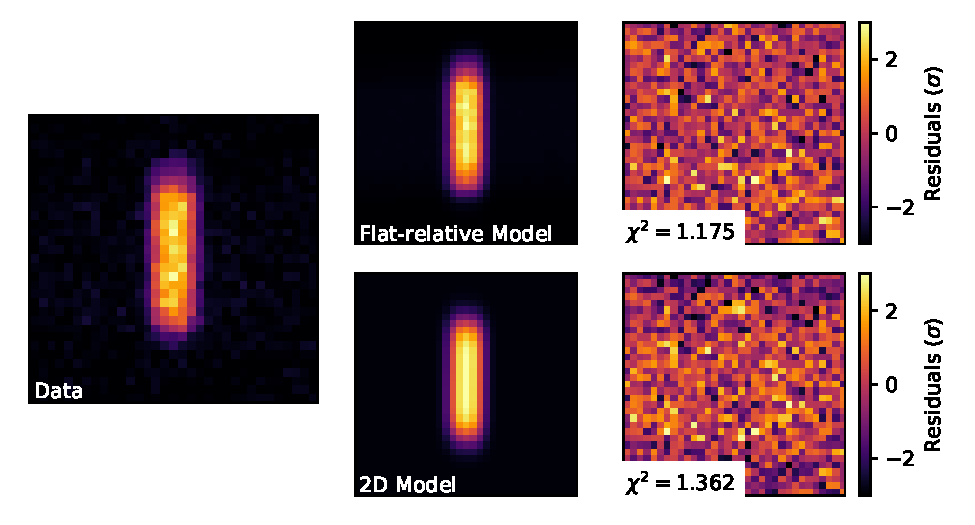
\includegraphics[width=\textwidth]{figures-5/expres-psf.pdf}
    \caption{Fit PSF model and residuals (along with corresponding $\chi^2$) using both the two-dimensional model (Equation \ref{eq:expres_psf}) and the flat-relative model (Equation \ref{eq:flat-relative-psf}).}
    \label{fig:psf-resid}
\end{figure}

In order to characterize the EXPRES PSF, I have implemented a Python sub-package within the EXPRES pipeline presented in Chapter \ref{chapter:pipeline}. This PSF sub-package uses a reduced observation of an emission line source to
\begin{enumerate}
    \item find the positions of individual emission lines, either universally or only along nightly traced orders,
    \item fit any arbitrary PSF function (including flat-relative varieties) to each emission line (see Figure \ref{fig:psf-resid}), masking severe pixel outliers (typically cosmic rays) and rejecting lines not fit well enough by the model (typically blended ThAr lines), and
    \item fit a two-dimensional polynomial (a $4 \times 4$ coefficient matrix with a Design Matrix structure as in Chapter \ref{wavelength-calibration}) to each of the PSF fit parameters, such that an interpolated PSF could be constructed for any pixel-position on the detector or for any pixel along a traced order (see Figures \ref{fig:psf-params-2d} and \ref{fig:psf-params-1d}).
\end{enumerate}
This code is relatively fast, able to map the PSF from a single image in less than two minutes using Equation \ref{eq:flat-relative-psf} and less than five minutes using Equation \ref{eq:expres_psf}.

\begin{figure}
    \centering
    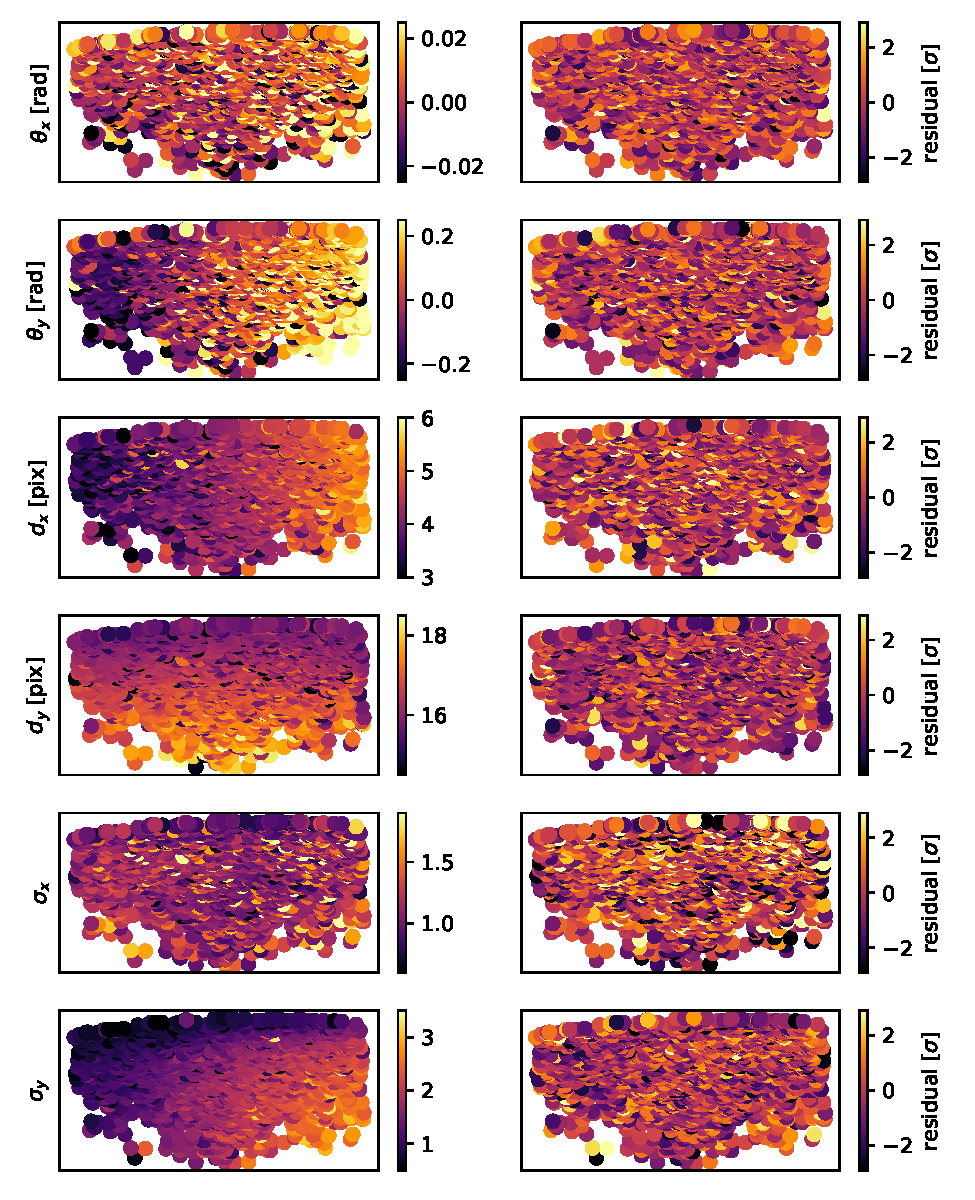
\includegraphics[width=\textwidth]{figures-5/psf-params-2d.pdf}
    \caption{PSF parameters from Equation \ref{eq:expres_psf} mapped across the detector using a ThAr observation from October 24, 2020. 1736 lines were fit using this method. Residuals from the 2D polynomial regression are presented alongside the parameters.}
    \label{fig:psf-params-2d}
\end{figure}

\begin{figure}
    \centering
    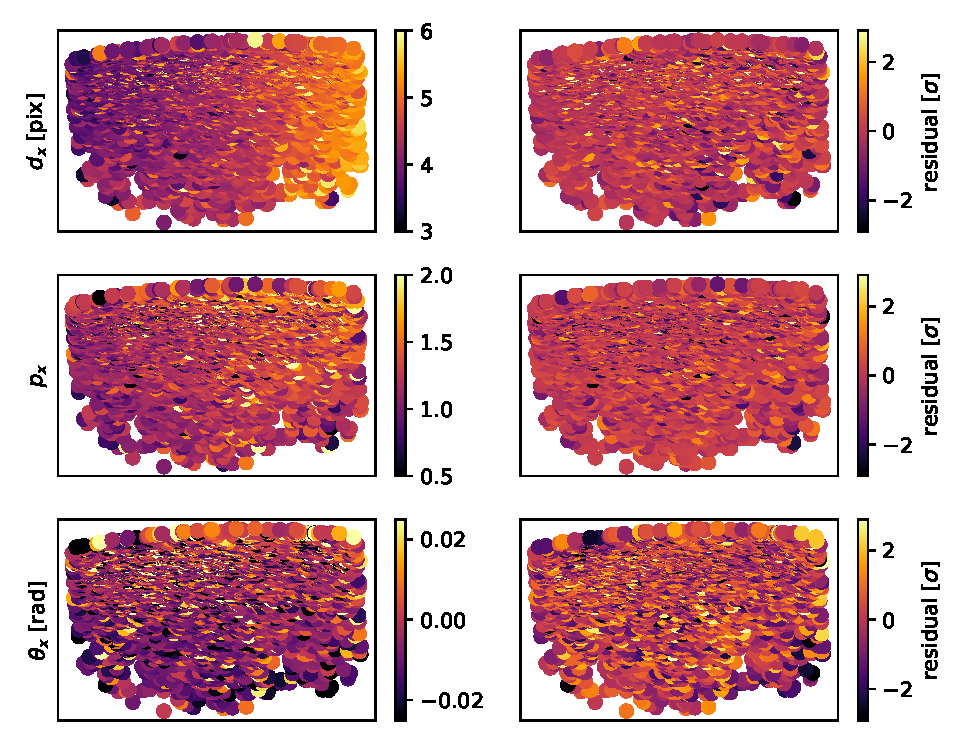
\includegraphics[width=\textwidth]{figures-5/psf-params-1d.pdf}
    \caption{PSF parameters from Equation \ref{eq:flat-relative-psf} mapped across the detector using a ThAr observation from October 24, 2020. 4367 lines were fit using this method. Residuals from the 2D polynomial regression are presented alongside the parameters.}
    \label{fig:psf-params-1d}
\end{figure}

Residual images for the two-dimenstional PSF model (Figure \ref{fig:psf-params-2d}) and the flat-relative model (Figure \ref{fig:psf-params-1d}) demonstrate how the parameters do vary smoothly across the detector and are accurately mapped by two-dimensional cubic polynomials with less than $3\sigma$ residuals. However, for the same ThAr observation, the flat-relative model rejected far fewer lines when fitting the model. This is likely due to aforemetioned degeneracies in Equation \ref{eq:expres_psf} and demonstrates the difficulty in developing a full two-dimensional PSF for an \'{e}chelle spectrograph.

Therefore, it is apparent that the flat-relative model has multiple advantages when characterizing the EXPRES PSF:
\begin{enumerate}
    \item use of the flat includes intrinsic detector structure in the model,
    \item fewer parameters means less computation time and model complexity,
    \item fewer lines are rejected during the regression, and
    \item flat-relative residuals are slightly better.
\end{enumerate}
Thus, for the EXPRES implementation of spectro-perfectionism, I moved forward with exclusively using the flat-relative approach.

\subsection{Implementation Considerations} \label{pipeline2:spec-perf:implement}

With knowledge of the basic spectro-perfectionism algorithm and a method to construct a flat-relative PSF, there are still a handful of other considerations to make when implementing these methods. In this section, I address processing resources, cosmic-ray rejection, and extraction sampling as they are key to putting it all together.

The most glaring issue with spectro-perfectionism is the sheer potential size of the arrays used in the deconvolution and reconvolution. Considering $\vb{\Psi}$ is meant to capture the full-detector contribution of the PSF at every sampling point of $\vb{s}$, this would yield a $N \times M \times L$ array where $N$ and $M$ are the dimensions of the detector and $L$ is the number of sampled points along the order. For EXPRES, each of these quantities are greater than 5,000, making this one array (using all floating point values) 2--3 TB in memory, obviously not possible with modern memory modules. Therefore, knowing that the PSF tails extremely quickly not far from its central point as noted in Chapter \ref{pipeline2:spec-perf:bkgd}, the memory footprint can be decreased significantly by only storing a small thumbnail image at each sampled point. For EXPRES, I have set the dimensions of this thumbnail to $33 \times 33$ pixels, leaving sufficient room for the approximately $16 \times 4$ pixel rectangular PSF.

Another important computational consideration relates to the complexity of matrix operations used in calculating Equation \ref{eq:convolution-soln} and the reconvolution matrix $\vb{R}$. Specifically, $\vb{\Sigma_s}^{-1}$ is an $L \times L$ matrix that needs to be eigen-decomposed, enabling trivial calculation of both the inverse and matrix square root. Eigen-decomposition has $\mathcal{O}(L^3)$ complexity, unfortunately, meaning this problem does not scale very well, especially if implementing increased spectral sampling as discussed later in this section. Thankfully $\vb{\Sigma}_{\vb{s}}^{-1}$ is symmetric and band-diagonal which enables some sparse-matrix speed-ups.

Similar to the PSF mapping algorithms, the EXPRES implementation of spectro-perfectionism is written as a Python sub-package within the EXPRES pipeline. The algorithms---especially the matrix inversion and eigenvalue decomposition---are accelerated using SciPy's sparse linear algebra functions \citep{virtanen_scipy_2020}. Even so, extraction of a single order at single pixel sampling can take almost 30 seconds, meaning extraction of a complete spectrum can take upwards of 45 minutes.

One possible speed up for the extraction, implemented by \citet{cornachione_full_2019} with Minerva-Red, is to run spectro-perfectionism on overlapping subsections of each order and then combine them after reconvolution. This can easily decrease the size of $L$ and therefore substantially increase the speed of the extraction. I would highly caution against this, however, due to ringing artifacts that can appear near the overlap points. Take, for example, Figure \ref{fig:spec-perf-ringing}, with an order extracted by spectro-perfectionism both in its entirety and in small chunks. Even though these two spectra appear very similar from a distance, looking at the normalized residuals between them,
\begin{equation}
    \sigma_{12} = \frac{s_1 - s_2}{\sqrt{\sigma_1^2 + \sigma_2^2}},
    \label{eq:residual}
\end{equation}
the spectra are clearly affected by this technique. Although the residuals are at the $1\sigma$ level for this example, they get worse when dividing the spectrum into even smaller chunks. Therefore, I maintain that each order of EXPRES is extracted in its entirety by the spectro-perfectionism algorithm.

\begin{figure}
    \centering
    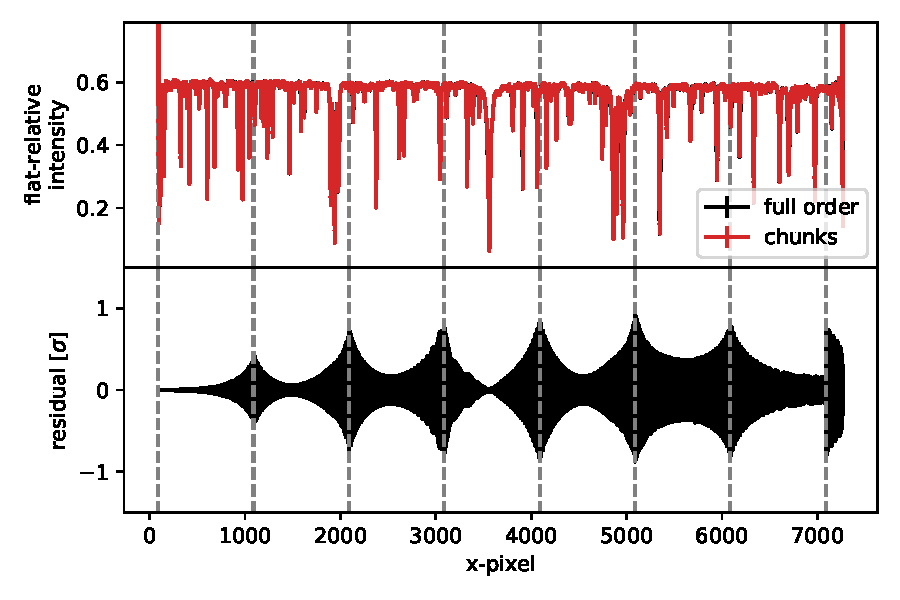
\includegraphics[width=\textwidth]{figures-5/spec-perf-ringing-1.pdf}
    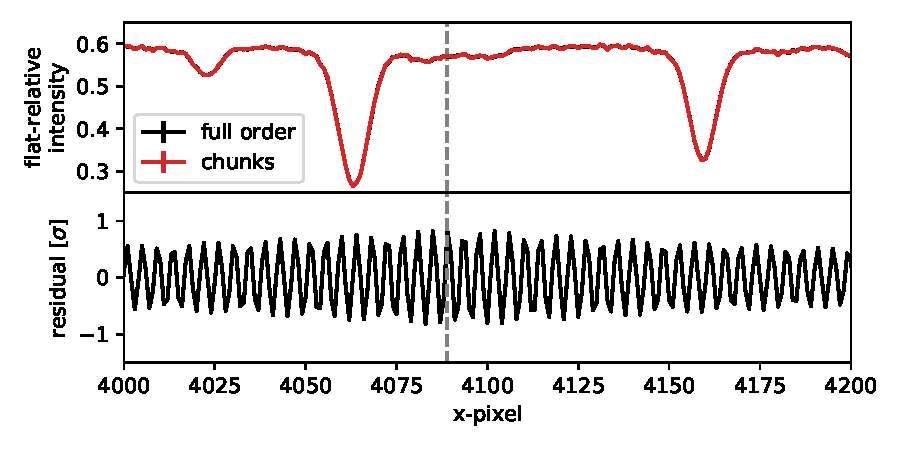
\includegraphics[width=\textwidth]{figures-5/spec-perf-ringing-2.pdf}
    \caption{HD 3651, absolute order 60, extracted by spectro-perfectionism over the full order as well as in 1000 pixel chunks padded by 200 pixels. The full order (top) and a zoomed region near one of the chunk boundaries (bottom) are shown. Ringing artifacts especially around the intersection points of adjacent chunks (marked by gray dashed lines) are readily apparent in the normalized residuals.}
    \label{fig:spec-perf-ringing}
\end{figure}

Cosmic ray rejection is built directly into the extraction algorithm, similar to EXPRES's implementation of optimal extraction (Chapter \ref{optimal-extraction}). After calculation of $\vb{s}$ as in Equation \ref{eq:convolution-soln}, a two-dimensional model of the order is generated and residuals for each pixel are calculated:
\begin{equation}
    r_{x,y} = \frac{D_{x,y} - \sum_\lambda{\Psi_{x,y,\lambda}s_\lambda}} {\Sigma_{x,y}^{-1/2}}.
    \label{eq:spec-perf-resid}
\end{equation}
All pixels with residuals greater than $5\sigma$ are masked from the data and the complete order is subsequently deconvolved again. In order to speed up this aspect of the pipeline, I only re-execute the deconvolution on portions of the CCD affected by cosmic ray masking in the previous iteration.

The final consideration is the choice of extraction sampling, since it also has implications for the computational complexity and the normalization of the flat-relative PSF. \textit{Sampling} in this context is simply the choice of how densely to extract a spectrum along a given order. Optimal extraction is limited to the horizontal pixel dimension of the detector: each spectral sample relates to one column of the detector. Spectro-perfectionism does not have this limitation since a 2D PSF could be centered on fractional pixels. Thus, there are many different ways in which a given order could be sampled. For simplicity in executing the algorithm and comparing it against optimal extraction as done in the following section, I will only present results here which have the same sampling density as optimal extraction: once per detector column. Arbitrary sampling densities, however, are still explorable with this implementation of spectro-perfectionism.

\subsection{Extraction Performance} \label{pipeline2:spec-perf:performance}

Using Equation \ref{eq:spec-perf-resid}, the modelling performance on a single order of the two PSF models, as well as that from optimal extraction, can be compared. This is visualized in Figure \ref{fig:extraction-residuals} for a small portion of a stellar observation order. Due to their ability to exactly match the cross-dispersion shape of the EXPRES PSF, flat-relative optimal extraction and flat-relative spectro-perfectionism perform equally well in extracting the data, especially along the trace of the order. The positive and negative residual arcs that follow along the top and bottom edges of the order are likely due to subtle vertical shifts in the order trace throughout the night \citep[significantly less than one pixel per day,][]{blackman_performance_2020}. However, their residuals are less than $1\sigma$ and therefore have little effect on the extracted spectrum, especially when compared to residuals from two-dimensional PSF models (which would also face the same misalignment).

\begin{figure}
    \centering
    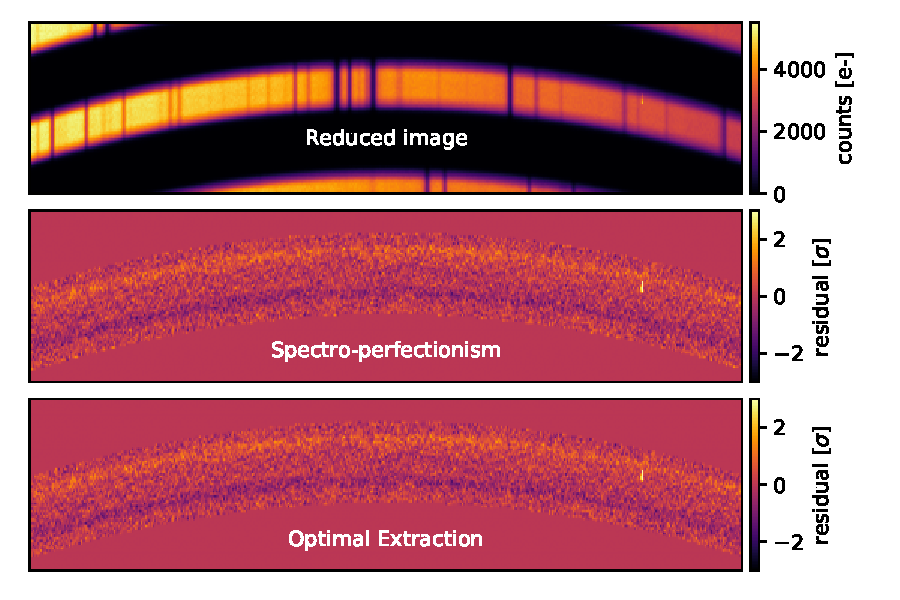
\includegraphics[width=\textwidth]{figures-5/extraction-residuals.pdf}
    \caption{Pixel-by-pixel extraction residuals for a section of relative order 60 of an observation of HD 3651 on October 24, 2020 (top) using both spectro-perfectionism (middle) and optimal extraction (bottom). Residuals here are normalized by the estimated noise model for each pixel.}
    \label{fig:extraction-residuals}
\end{figure}

The similarities between spectro-perfectionism and optimal extraction also extend into the extracted spectra. As shown in Figure \ref{fig:spec-perf-vs-optimal}, the two spectra nearly exactly align with normally-distributed residuals (see Equation \ref{eq:residual}). The total reduced $\chi^2$ for this order is 1.14. Notice, however, that the residuals do spike ever-so-slightly around the sides of deep stellar lines. There is likely some different information being extracted in these regions with the two-dimensional PSF.

\begin{figure}
    \centering
    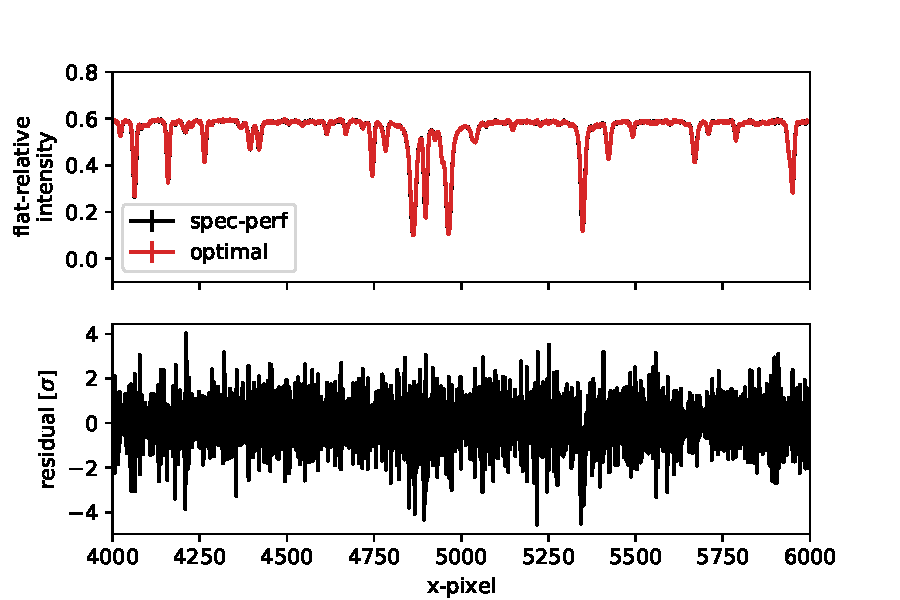
\includegraphics{figures-5/spec-perf-vs-optimal.pdf}
    \caption{Comparison of spectro-perfectionism against optimal extraction for an extracted spectrum using the same data as in Figure \ref{fig:extraction-residuals}.}
    \label{fig:spec-perf-vs-optimal}
\end{figure}

Differences in the method are much more apparent, however, when extracting observations of an emission line source, such as an LFC, with spectro-perfectionism. As shown in Figure \ref{fig:spec-perf-vs-optimal-lfc}, the individual lines are are ``peakier'' (brighter peaks, smaller line widths) when using spectro-perfectionism, implying higher resolution and signal-to-noise. However, this appears to come with a cost: some of the ringing from the deconvolution has remained even after reconvolution, as evidenced by the two ``lobes'' that appear equally spaced between each LFC line. This exact same structure (with either one or two lobes between each line) even occurs when using simulated ``perfect'' LFC lines with no background, indicating that the lobes are not caused by true signal between LFC lines. The issue seems to lie with the choice of reconvolution matrix, which will unfortunately require further exploration to resolve.

\begin{figure}
    \centering
    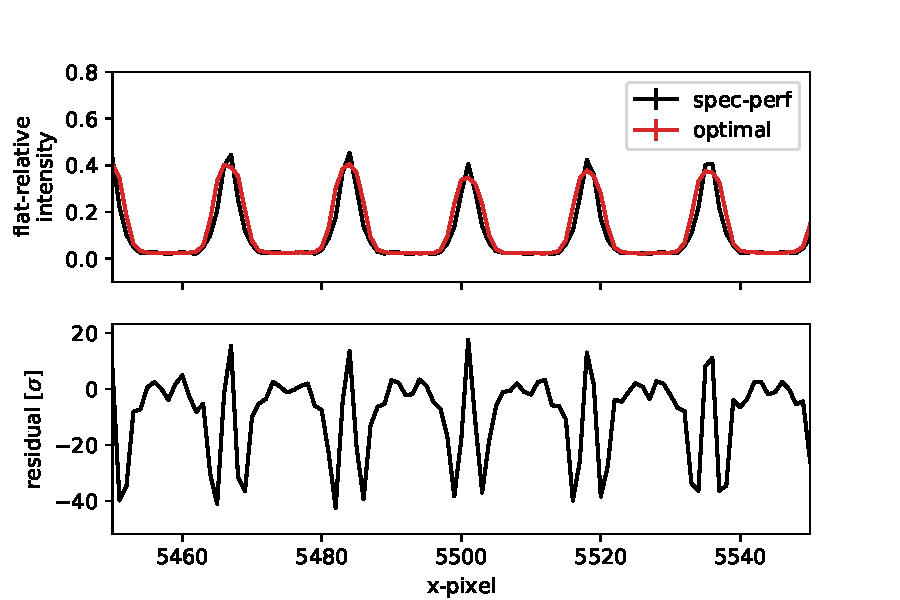
\includegraphics{figures-5/spec-perf-vs-optimal-lfc.pdf}
    \caption{Comparison of spectro-perfectionism against optimal extraction for an extracted spectrum of an LFC, taken on the same date as the data in Figure \ref{fig:spec-perf-vs-optimal}.}
    \label{fig:spec-perf-vs-optimal-lfc}
\end{figure}

Regardless, the ultimate test of spectro-perfectionism is its ability to accurately measure RVs. Between August 19, 2019, and January 31, 2021, EXPRES took [INSERT NUMBER] of observations of HD 3651. I extracted these observations with both flat-relative spectro-perfectionism and the default flat-relative optimal extraction of the EXPRES pipeline. Due to the aforementioned issue with emission line sources and to decrease total computation time, I generated wavelength solutions for each set using only the optimally-extracted calibration sources, meaning the only difference in the two data sets is the method of extraction. Results from this test are visualized in Figure \ref{fig:spec-perf-rvs} and orbital parameters are summarized in Table \ref{tab:spec-perf-rvs}.



\begin{figure}
    \centering
    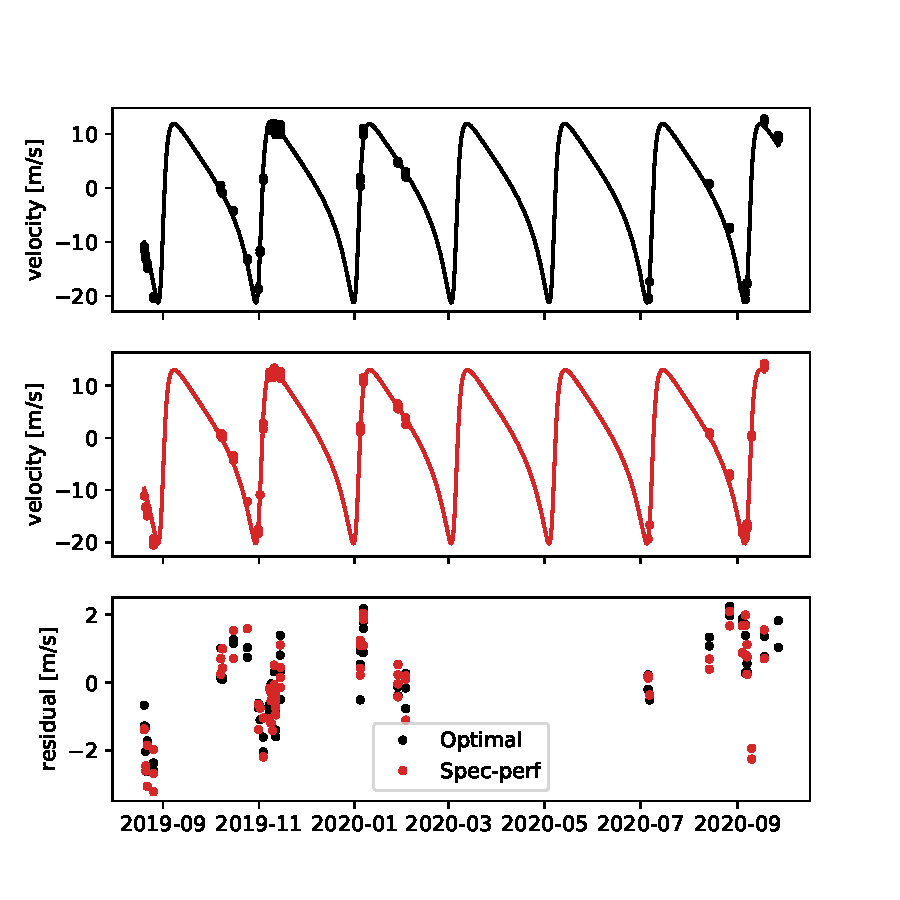
\includegraphics{figures-5/spec-perf-rvs.pdf}
    \caption{RVs generated from the EXPRES pipeline after using both optimal extraction and spectro-perfectionism on a series of HD 3651 observations. Residuals from fit Keplerian models for each set of RVs are shown in the bottom plot.}
    \label{fig:spec-perf-rvs}
\end{figure}

\begin{table}[width=\textwidth]
    \centering
    \begin{tabular}{lll}
        \hline
        \hline
        Parameter & Spec-perf & Optimal \\
        \hline
        $K$ [\ms] & & \\
        $P$ [days] & & \\
        $e$ & & \\
        RMS [\ms] & & \\
    \end{tabular}
    \caption{Keplerian orbital parameters of HD 3651 b}
    \label{tab:spec-perf-rvs}
\end{table}

\subsection{Discussion}

There is much left to be explored and improved with spectro-perfectionism.

EXPRES has an advantage over other RV spectrographs which makes flat-relative spectro-perfectionism (and even, by extension, optimal extraction) more accurate: a rectangular fiber input. One of the largest improvements from using a flat-relative PSF---less complexity in the model---could be completely removed from a less separable PSF function. Take, for example, a circular or elliptical PSF. 

Gold deconvolution

Magain sampling

\section{\textit{B}-spline Regression} \label{pipeline2:bspline}

There are two distinct ways to think about and work with a spectrum after it has been extracted from an \'{e}chelle spectrograph and wavelength calibrated: (1) order-wise and (2) continuously. When dealing with a spectrum order-wise, each \'{e}chelle order is treated as functionally independent, essentially as if the end-user has 86 individual spectra to work with. This is the default behavior of the EXPRES Pipeline (Chapter \ref{chapter:pipeline}) for everything post-extraction: continuum normalization, telluric modelling, and RV analysis.

However, neighboring orders of EXPRES spectra actually overlap in wavelength significantly, meaning that a single continuous spectrum could be generated across the entire band-pass of the instrument. This is further enabled by the fact that flat-relative optimal extraction yields the same spectral output for a given wavelength regardless of which order it came from. To have the same output with a typical optimal extraction would require fitting and dividing out the blaze before combining orders, a potentially dubious process \citep{xu_modeling_2019}.

Combining orders in such a way helps by increasing signal-to-noise along the edges of each order, where the blaze function is dimmest. Since the light in these regions is shared between adjacent orders, it is beneficial to combine these signals in such a way to improve the overall fidelity of the spectrum. Overlapping ends of adjacent orders, however, do not have equivalent wavelengths sampling. Therefore, combining this data is not as simple as taking a weighted mean of spectral data at a given wavelength. Rather, the data would need to be resampled to a single wavelength grid \citep{anglada-escude_harps-terra_2012} or regressed with a smoothing function.

\textit{B}-splines \citep{de_boor_practical_1978, dierckx_curve_1995, eilers_flexible_1996} are powerful smoothing functions that can be applied specifically for this purpose. A \textit{B}-spline is a piece-wise polynomial function of order $n$ made up of a linear combination of $K$ knots ($k$) each weighted by their own coefficient $c_k$
\begin{equation}
    F(x,{c_k}) = \sum_k {c_k B_{k,n}(x)}
\end{equation}
where $B_{k,n}$ are degree-$n$ basis functions of the \textit{B}-spline defined using the Cox-de Boor recursion formula \citep{de_boor_practical_1978}. $B$-splines are advantageous primarily because they can be expressed as a linear least-squares problem: uncertainties in the data are folded directly into the analysis and the regression can be run quickly even with a large amount of data, Also, the knots of a $B$-spline can be arbitrarily chosen, meaning that the ``sampling'' of this smoothing function can be chosen relative to the sampling of the instrument, whether that be undersampling to provide an estimate for the continuum, matching instrument sampling to combine orders, or oversampling when co-adding spectra to increase template resolution.

Within this section, I use the term \textit{resolution knots} to described \textit{B}-spline knots that are equally spaced by resolution, or that $\frac{\lambda_k}{\Delta \lambda_k}$ is held constant for each adjacent pair of knots. With some inspection, you'll notice that this simply means the logarithmic wavelengths of the knots are spaced equally. However, I choose to describe the ``resolution'' of the knots as a more intuitive way of understand how they are spaced within the spectrum. For example, $R=137,500$ knots would exactly match the resolution of EXPRES (one knot approximately every four pixels) while $R=600,000$ knots would be clearly oversampling the instrument with a knot essentially at each pixel.

In this section, I provide two use cases for $B$-spline regression within the EXPRES pipeline: continuum normalization (Chapter \ref{pipeline2:bspline:cont-norm}), which has already been implemented as default behaviour in the pipeline, and stellar templating (Chapter \ref{pipeline2:bspline:templates}) which provides options for combining orders and telluric modeling. In Chapter \ref{pipeline2:forward-model}, I describe how these stellar templates are used as a forward model to generate alternative RVs for EXPRES.

\subsection{Continuum Normalization} \label{pipeline2:bspline:cont-norm}

An important property of the flat-relative optimal extraction used in the EXPRES pipeline (Chapter \ref{optimal-extraction}) is that the extracted continuum across the entire spectrum is a continuous and smooth function. This smoothness enables the use of an order-wise linear regression in the previously described pipeline, but the continuity can be leveraged to easily enhance continuum normalization with the use of a $B$-spline regression for the entire spectrum.

\begin{figure}
    \centering
    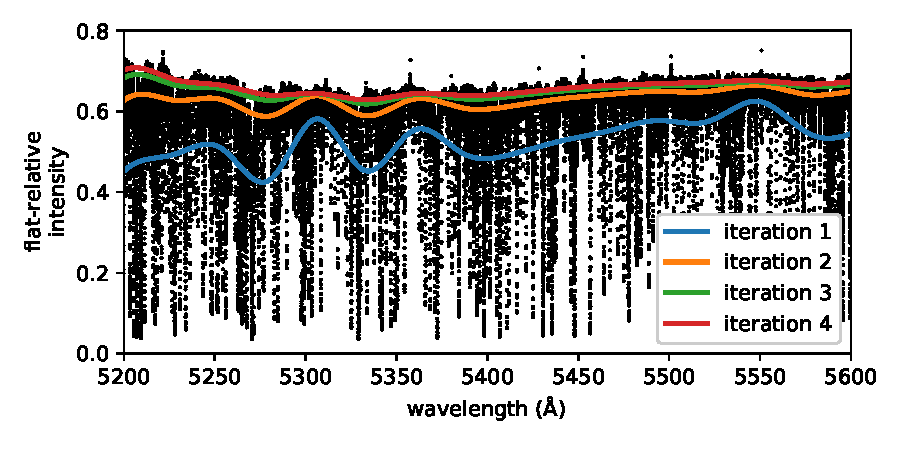
\includegraphics[width=\textwidth]{figures-5/cont-norm-bspline.pdf}
    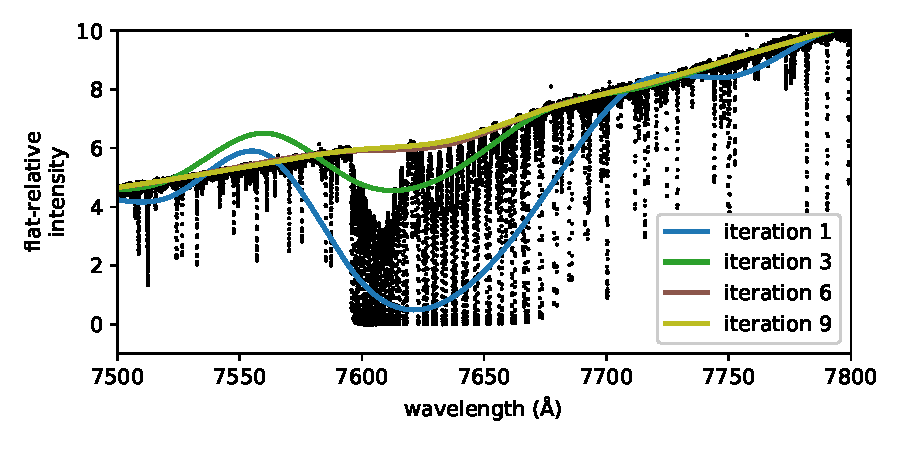
\includegraphics[width=\textwidth]{figures-5/cont-norm-bspline-oxygen.pdf}
    \caption{Iterative technique of absorption line rejection using a full-spectrum \textit{B}-spline regression shown for two separate regions of an HD 3651 spectrum. The bottom plot specifically shows the oxygen a-band, Which crosses between \'echelle orders 80 and 81, and is well-characterized by the \textit{B}-spline continuum.}
    \label{fig:cont-norm-bspline}
\end{figure}

To fit the continuum, I use an $R=100$ knot spacing and cubic ($n=2$) \textit{B}-spline basis functions. The same iterative technique of outlier rejection for absportion lines, now with a $-1.5\sigma$ cut-off, can be applied after each regression to slowly morph the \textit{B}-spline to the continuum of the spectrum. The resultant continuum at each step of this iterative process is shown in Figure \ref{fig:cont-norm-bspline}.

The improvements with using a continuous $B$-spline regression rather than the order-wise linear fit is most apparent for \'{e}chelle orders 80 and 81 where the oxygen a-band is shared between the two orders. As also shown in Figure \ref{fig:cont-norm-bspline}, the continuum in this region is certainly not perfectly linear and is better described by the local cubic function. The large gaps in the continuum are easily handled by the \textit{B}-spline as well.

\subsection{Stellar Templates} \label{pipeline2:bspline:templates}

This \textit{B}-spline regression can also be used to combine (or ``co-add'') multiple observations of the same stellar target together to produce a resultant template at higher signal-to-noise and resolution as compared to a single observation. As opposed to the morphed SOAP solar spectrum presented as the forward model in Chapter \ref{forward-modeling}, such a stellar template would be completely empirical and could precisely detail the nuances of both the absorption lines and the varying PSF of the instrument. No assumptions could be made about the spectra before combining them, enabling a completely data-driven approach to modeling the spectra.

Of course, multiple considerations need to be made before I can simply stack the observations on top of each other and fit them with a \textit{B}-spline:
\begin{enumerate}
    \item the spectra must be barycentric corrected to ensure they are not offset by 10's of km/s,
    \item planet-imposed stellar radial velocities could offset these spectra by 10's of m/s, and
    \item telluric contamination must be either masked or divided out in each co-added spectrum.
\end{enumerate}
Barycentric correction (1) is an inherent part of the pipeline so these large offsets are automatically corrected for. And, considering a single pixel on the EXPRES detector corresponds to approximately 500 m/s in velocity space ($R = \frac{\lambda}{\Delta\lambda} = \frac{c}{\Delta v}$), typical planetary signals (2) will not affect the data significantly enough to prevent fitting a template. Telluric modeling (3), however, requires a bit more decision-making. In this case, I chose to mask all telluric lines with a depth greater than 0.1 (or a normalized spectral value less than 0.9) and divided out the rest, inflating the corresponding uncertainties accordingly. An example of a \textit{B}-spline stellar template for 95 combined observations of HD 3651 is shown in Figure \ref{fig:stellar-template}. 

\begin{figure}
    \centering
    \includegraphics[width=\textwidth]{figures-5/stellar-template.pdf}
    \caption{Portion of a stellar template generated from 95 observations of HD 3651. The tellurics are left in the data to demonstrate how they do not effect the eventual template.}
    \label{fig:stellar-template.pdf}
\end{figure}

\subsection{Discussion}

The use of \textit{B}-spline regression has proven useful throughout the EXPRES pipeline. It has shown high fidelity at modeling the continuum and co-adding full spectra. There are also numerous applications to the use of these templates. For example, I am currently working on a full-spectrum telluric model code based on the order-wise algorithms developed for SELENITE \citep{leet_toward_2019}. Also, combining orders and co-adding spectra could be used to generate higher signal-to-noise indicators for stellar activity, especially in the dimmest parts of the stellar spectra around the calcium H and K lines. Finally, as I describe in the following section, co-added spetra can be used as a forward model when measuring radial velocities.

One major downside of using \textit{B}-spline regression is the lack of a simple model for posterior uncertainty. \citet{zechmeister_spectrum_2018} provide error estimates for the coefficient at each knot, which can be subsequently propagated, but these are extremely simplified and may dilute a true error analysis. Some alternatives do exist \citep{enting_propagating_2006, gardner_uncertainties_2003}, but their implementation are outside the scope of this work. Regardless, since the main application of the \textit{B}-spline regression in this context is as a model (for continuum, tellurics, or full spectra), the uncertainty can be assumed negligible.

An important caveat to the use of a spectrum continuously, rather than order-wise, is the fact that order-to-order spectral matching is not absolutely perfect, even when using a flat-relative optimal extraction. Since the PSF is spread across a different number of pixels on the left and right side of each order (i.e. the dispersion is not constant), there are slightly different relative contributions to a given spectral bin. An example of this is shown in Figure \ref{fig:order-matching} for a few concurrent orders of HD 3651. Note that the effect rarely produces more than $1\sigma$ residual, meaning the effect is small, but still clearly systematic. Flat-relative spectro-perfectionism could provide a solution to this issue, but it would require matching the local sampling of the PSF to the dispersion of the instrument which subsequently requires precise matching of normalization factors to each spectral bin.

\begin{figure}
    \centering
    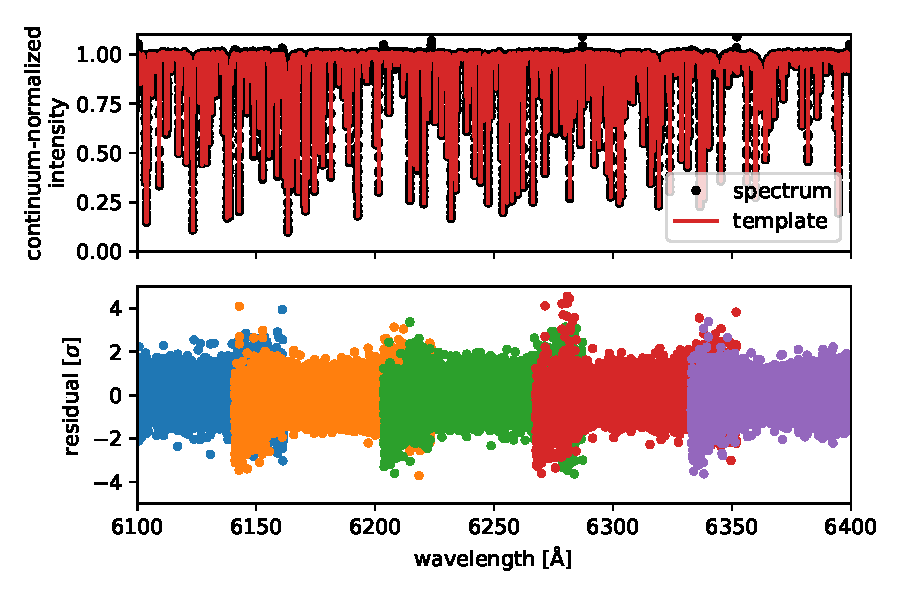
\includegraphics{figures-5/order-matching.pdf}
    \caption{Overlapping spectral orders of an observation of HD 3651 and the resultant residuals to the \textit{B}-spline regression. Each \'{e}chelle order in the residual plot is colored differently to emphasize the trend. This effect is seen for all observations made with EXPRES, including wavelength calibrations.}
    \label{fig:order-matching}
\end{figure}

A strong alternative to \textit{B}-spline regression could be Gaussian Process (GP) Regression \citep{rajpaul_robust_2020} due to its intrinsic ability to model uncertainty and availability of a wide variety of viable kernels to appropriately smooth the data. That being said, GPs do not scale very well, even beyond just a few hundred data points, meaning modern computational resources would not be able to come close to co-adding multiple spectra simultaneously. A spectrum from EXPRES modeled with a GP, for example, would require hundreds of separate ``chunks'' that would need to be spliced together. Thus, despite its drawbacks, I still highly recommend the use of \textit{B}-splines when combining spectral data, especially because of its speed and ability to carefully define a model resolution through knot locations.

\section{\textit{B}-spline Forward Model RV Measurement} \label{pipeline2:forward-model}

With a \textit{B}-spline stellar template in hand, I constructed a forward modeling algorithm distinct from but similar to the one presented in Chapter \ref{forward-modeling}. The primary changes within this new analysis are:
\begin{itemize}
    \item it is written in Python for simpler integration with the rest of the EXPRES pipeline,
    \item it makes use of the \textit{B}-spline stellar templates,
    \item it can optionally set the chunks to use \textit{wavelength} bins as opposed to \textit{pixel} bins.
\end{itemize}
This final point is most critical to the new implementation; since the \textit{B}-spline makes use of the full spectrum simultaneously as opposed to order-wise, it follows that the RV analysis could do the same. This enables the same benefit as for combining orders in other analysis---increased signal-to-noise along the ends of orders---which should enable greater consistency in RV measurement for these particular regions of the spectra.

The chunk-by-chunk velocity measurement is similar to that used in the previous chunk-by-chunk analysis:
\begin{enumerate}
    \item combine all observations of the given stellar target, mask out telluric lines deeper than half the continuum and divide the given telluric model for shallower lines,
    \item use the above \textit{B}-spline regression to generate a template for the stellar target,
    \item set boundaries for chunks across the target spectrum, whether that be equal in pixels along each order (I use 100-pixel chunks) or equal in wavelength bins (I use 1~nm chunks), and
    \item run a least squares fit on each target chunk by varying the velocity offset in the wavelengths of the template, iteratively masking $5\sigma$ outliers.
\end{enumerate}
Masked residual outliers in the spectrum typically come from improper telluric modeling. An example of chunk velocities for HD 3651 are shown in Figure \ref{fig:chunk-vels} for both pixel- and wavelength-chunks.

\begin{figure}
    \centering
    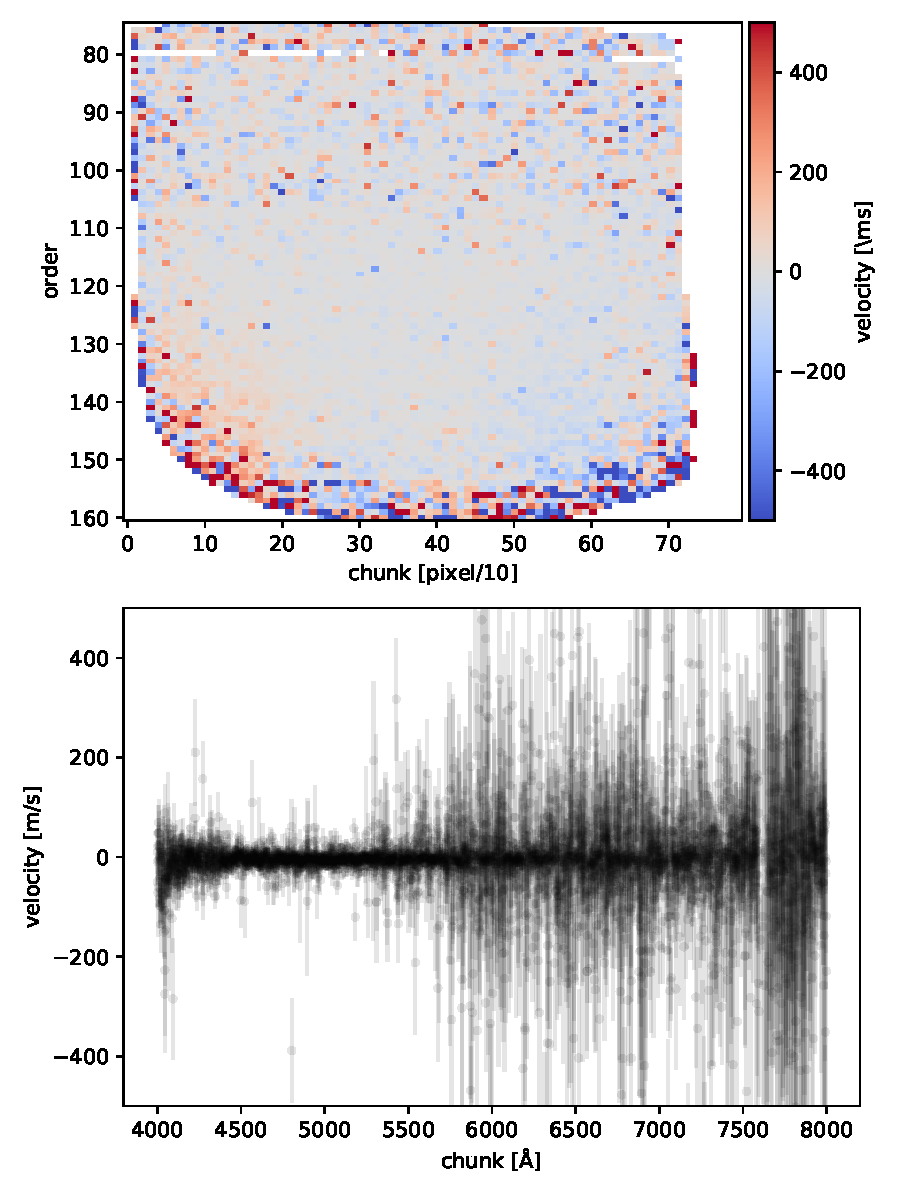
\includegraphics{figures-5/chunk-vels.pdf}
    \caption{Demonstration of chunk velocities for an observation of HD 3651 taken on October 24, 2020 using both pixel-chunks (left) and wavelength-chunks (right).}
    \label{fig:chunk-vels}
\end{figure}

Once a velocity and uncertainty is generated for each chunk, an RV for the observation can be calculated:
\begin{enumerate}
    \item calculate the variance weighted mean for each observation,
    \item calculate a variance weighted mean residual for each chunk (an approximation for the systematic velocity offset of the chunk) and subtract it from each corresponding chunk velocity of each observation,
    \item calculate a reduced $\chi$ metric for each chunk (a normalized approximation for the intrinsic velocity scatter of the chunk) and multiply it against each corresponding chunk uncertainty of each observation, and
    \item re-calculate the variance weighted mean for each observation, iteratively masking $5\sigma$ outliers one by one.
\end{enumerate}
These steps are meant to mitigate systematic effects due to the instrument (e.g. detector non-uniformities), stellar activity which may modify certain absorption lines more than others, and possible residual problems due to imperfect telluric modeling. An example of the systematic velocity offsets and reduced $\chi$ metric for each chunk is shown in Figure \ref{fig:chunk-offsets}.

\begin{figure}
    \centering
    \includegraphics{figures-5/chunk-offsets.pdf}
    \caption{Chunk mean velocity offsets (left) and reduced $\chi$ metrics (right) over all observations of HD 3651.}
    \label{fig:chunk-offsets}
\end{figure}

The data set used to compare against previous RV measurement methods is the same as used for spectro-perfectionism: observations of HD 3651 from [DATE] to [DATE]. A comparison of the velocities generated from the previous and this new forward model are shown in Figure \ref{fig:cbc-comparison} along with corresponding residuals to a Keplerian orbital fit. [ANALYSIS HERE]

\begin{figure}
    \centering
    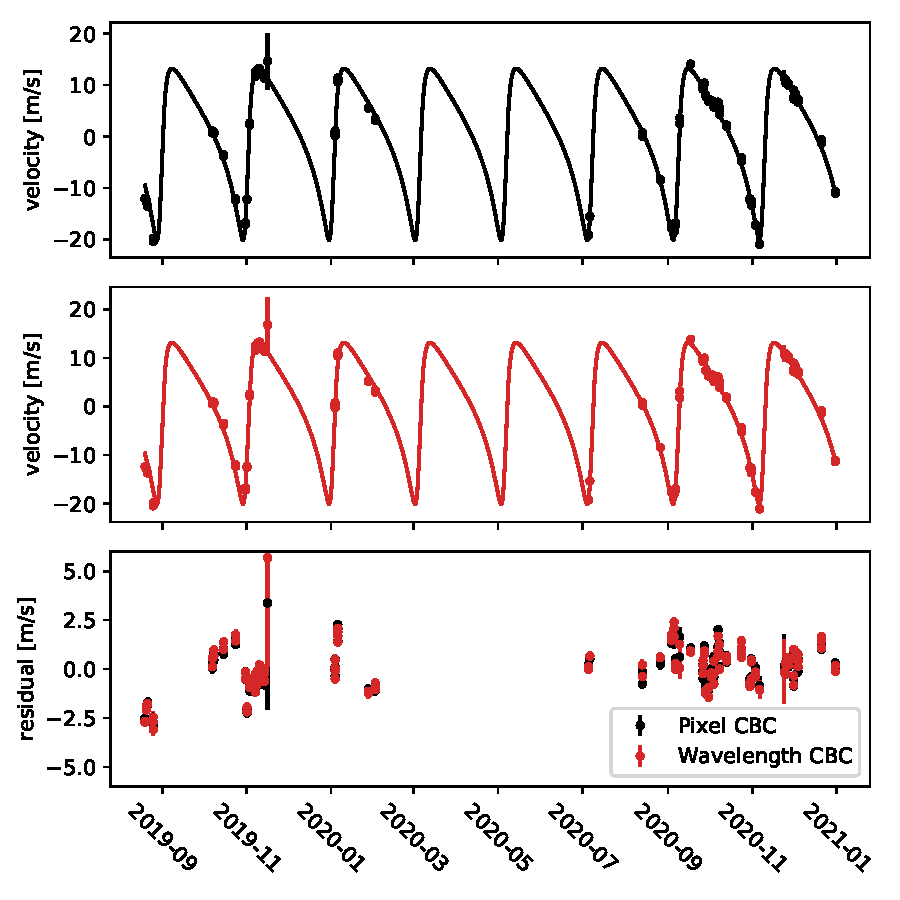
\includegraphics{figures-5/cbc-comparison.pdf}
    \caption{Comparison of the two chunk-by-chunk velocities and corresponding residuals to a Keplerian orbital fit.}
    \label{fig:cbc-comparison}
\end{figure}

\begin{table}[width=\textwidth]
    \centering
    \begin{tabular}{llll}
        \hline
        \hline
        Parameter & Old CBC & New CBC & CBC WVLN \\
        \hline
        $K$ [\ms] & & & \\
        $P$ [days] & & & \\
        $e$ & & & \\
        RMS [\ms] & & & \\
    \end{tabular}
    \caption{Keplerian orbital parameters of HD 3651 b}
    \label{tab:spec-perf-rvs}
\end{table}


\section{Summary and Discussion} \label{pipeline2:discussion}

Spectro-perfectionism and \textit{B}-spline regression have both proven to be quite fruitful avenues of exploration at advancements to the EXPRES pipeline.




I would like to thank Joel Ong for introducing me to spectro-perfectionism and providing some of the groundwork on developing the deconvolution algorithms. I would also like to thank Adam Bolton for his conversations on this fascinating topic.

